\documentclass{article}
\usepackage[T1]{fontenc}
\usepackage[utf8]{inputenc}

\usepackage{cmbright}
\usepackage[T1]{fontenc}

\usepackage{multicol}

\usepackage{amsmath}
\usepackage{amsfonts}
\usepackage{amssymb}
\usepackage{tikz}
\usepackage{graphicx}
\graphicspath{  {./images/} }
\setlength{\parindent}{0pt}
\usepackage{changepage}
\usepackage{verbatim}
\usepackage{physics}
\usepackage{derivative}
\usepackage{bm}
\usepackage[colorlinks=true, linkcolor=blue, urlcolor=blue, citecolor=blue, anchorcolor=blue]{hyperref}

\addtolength{\oddsidemargin}{-.25in}
\addtolength{\textwidth}{0.5in}

\makeatletter
\newcommand*\bigcdot{\mathpalette\bigcdot@{.5}}
\newcommand*\bigcdot@[2]{\mathbin{\vcenter{\hbox{\scalebox{#2}{$\m@th#1\bullet$}}}}}
\makeatother

\DeclareMathOperator{\di}{d\!}
\newcommand*\Eval[3]{\left.#1\right\rvert_{#2}^{#3}}

\newcommand{\uvec}[1]{\boldsymbol{\hat{\textbf{#1}}}}
\newcommand{\vr}[1]{\textbf{#1}}

\newcommand{\thus}[0]{\; \; \longrightarrow \; \;}

\newcommand{\lag}{\mathcal{L}}
\newcommand{\ham}{\mathcal{H}}

\title{Spin Distribution Calculations}
\author{Ryan Liu}
\date{Last updated: July 20, 2021}

\begin{document}

\maketitle

\section{Resources Used}

\begin{itemize}
    \item Hartle \textit{Gravity} Chapter 15 (notes on Kerr Geometry and rotating black holes)
    \item LIGO Scientific Collaboration. \textit{Population Properties of Compact Objects from the Second Ligo-Virgo Gravitational Wave Transient Catalog.} \url{https://arxiv.org/abs/2010.14533}
    \item S Miller, T Callister, W Farr. \textit{The Low Effective Spin of Binary Black Holes and Implications for Individual Gravitational-Wave Events.} \url{https://arxiv.org/abs/2001.06051}
    \item Thibault Damour. \textit{Coalescence of Two Spinning Black Holes: An Effective One-Body Approach.} \url{https://arxiv.org/abs/gr-qc/0103018}
    \item P Schmidt, F Ohme, M Hannam. \textit{Towards models of gravitational waveforms from generic binaries II: Modelling precession effects with a single effective precession parameter}. \url{https://arxiv.org/abs/1408.1810}
\end{itemize}

\section{Notes}

The spacetime metric of a rotating black hole with mass \textit{M} and angular momentum \textit{J} is given by \textbf{Kerr Geometry}: 
\begin{equation}
    \begin{aligned}
        ds^2 = &-\Big(1 - \frac{2Mr}{\rho^2} \Big) dt^2 - \frac{4M ar \sin^2 \theta}{\rho^2} d\phi dt + \frac{\rho^2}{\Delta} dr^2\\
        & + \rho^2 d\theta^2 + \Big( r^2 + a^2 + \frac{2Mra^2 \sin^2 \theta}{\rho^2} \Big) \sin^2 \theta d \phi^2
    \end{aligned}
\end{equation}
where
\begin{equation}
    a \equiv J/M, \quad \rho^2 \equiv r^2 + a^2 \cos^2 \theta, \quad \Delta \equiv r^2 - 2Mr + a^2
\end{equation}
The parameter $a$ is known as the \textbf{Kerr parameter}, and is also the relative magnitude of spin reported by LIGO. Singularities occur when $\rho$ or $\Delta$ vanishies, as evident by (1). The singularity at $\rho$ occurs when $r = 0$ and $\theta = \pi/2$, which is simply the center of the black hole. Meanwhile, $\Delta$ vanishes at 
\begin{equation}
    r_\pm = M \pm \sqrt{M^2 - a^2}
\end{equation}
for $a \leq M$. We can observe that $r_+ = 2M$ when $a=0$, which corresponds to the zero-spin Schwarzchild metric. Qualitatively, we find that the greater the value of $a$, the greater the vertical ``squashing" of the black hole. \\

In measuring the spin from black holes, we consider two parameters -- the \textbf{effective spin} and the \textbf{effective precession spin}, which accurately predict the amplitude and phase evolution of a BBH merger. They are defined as 
\begin{gather}
    \chi_\text{eff} = \frac{\chi_1 \cos \theta_1 + q \chi_2 \cos \theta_2}{1 + q} \\
    \chi_\text{p} = \max \Big[ \chi_1 \sin \theta_1, \; \Big(\frac{4q + 3}{4 + 3q} \Big) q \chi_2 \sin \theta_2 \Big]
\end{gather}
where $\chi_1$ and $\chi_2$ are the spin magnitudes of $m_1$ and $m_2$ respectively ($m_1 \leq m_2$), $q \equiv m_2 / m_1$, and $\theta_1$ and $\theta_2$ are the misalignment angles between teh component spins and the orbital angular momentum of the BBH. 

\section{Calculations}

Because spin affects GW strength less than mass or distance, there is greater uncertainty in the spin distribution of BBH mergers for both $\chi_\text{eff}$ and $\chi_\text{p}$. \\

Based on an analysis of BBH mergers from both iLIGO and aLIGO, Abbott et al. proposes a \textit{Gaussian model} of $p(\chi_\text{eff})$ for the probability distribution of effective spins:
\begin{equation}
    p(\chi_\text{eff} | \mu, \sigma) = \mathcal{N} (\mu, \sigma) \text{exp} \Big[ \frac{-(\chi_\text{eff} - \mu)^2}{2\sigma} \Big]
\end{equation}
with parameters
\begin{equation}
    \mu_\text{eff} = 0.06_{-0.05}^{+0.05}, \quad \sigma_\text{eff} = 0.12_{-0.04}^{+0.06}
\end{equation}
where $\mu$ is the mean, $\sigma$ is the standard deviation, and $\mathcal{N}$ is the normalization constant. This is in agreement with the analysis of ten O1 and O2 events presented by Miller et al., which proposes the parameters
\begin{equation}
    \mu_\text{eff} = 0.02_{-0.13}^{+0.11}, \quad \sigma_\text{eff} \leq 0.07
\end{equation}
However, different conclusions are drawn -- whereas Miller et al. suggests that the spin distribution is undistinguishable from a delta function, Abbott et al. calculations that the fraction of binaries with positive spins, negative spins, and vanishingly small spins ($|\chi_\text{eff}| \leq 0.01$) are
\begin{equation}
    f_p = 0.67_{-0.16}^{+0.16}, \quad f_n = 0.27_{-0.15}^{+0.17}, \quad f_v = 0.05_{-0.01}^{+0.02}
\end{equation}
respectively. Given that Abbott et al. had the benefit of four times the number of BBH observations, we use the Gaussian model described in Eq. (7). \\

The distribution of $\chi_\text{p}$ has much greater uncertainity -- Abbott et al. states that using a Gaussian model, $\chi_\text{p}$ peaks at 0.2 but is \textit{either} broad or narrowly peaked (no estimates of $\sigma_\text{p}$ are given). For the following analysis, we (arbitrarily) choose an effective precession spin of 

\section{Results}

From Section (3.7), we were able to see that the main effect of the $z$-component spin was to dilate the GW signal in the time domain, with greater positive spins associated with longer signals and higher SNR. Using \texttt{IMRPhenomPv2}, we are able to repeat the same analysis for precession spin. 

\begin{figure}[!htb]
    \center{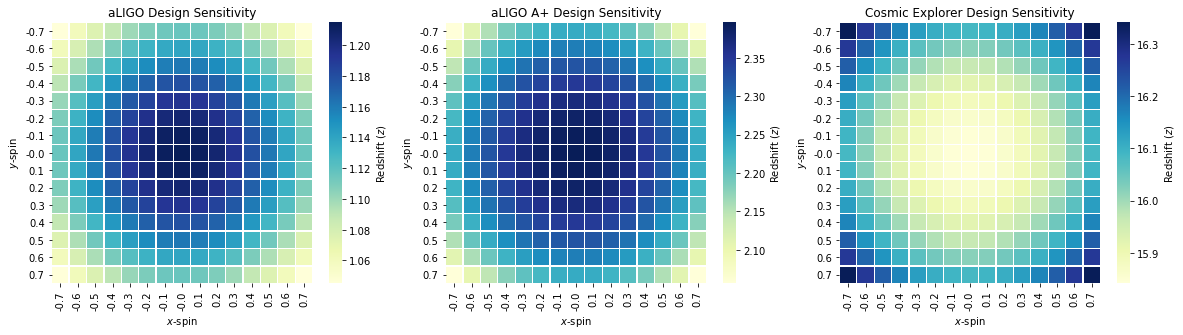
\includegraphics[width=\textwidth]{SNR30.png}}
    \caption{\label{fig:zchip} Maximum redshift of detection for a BBH of $m_1 = m_2 = 30 M_\odot$, assuming an aligned spin of $0$ and varying precession spin for $m_1$.}
\end{figure}

From Figure \ref{fig:zchip}, we see that for all three, there is a symmetrical effect on the GW signal strength between the $x$ and $y$ components, as expected. Thus, for all future calculations, the precession spin is assumed to be composed solely by the $x$ component of spin and positive. However, whereas lower precession spin magnitudes are associated with a stronger GW signal for aLIGO and A+ LIGO, an opposite effect is seen for Cosmic Explorer. This is likely because at high redshifts, the main determinant of GW signal strength becomes its length, rather than amplitude. \\

\begin{figure}[!htb]
    \center{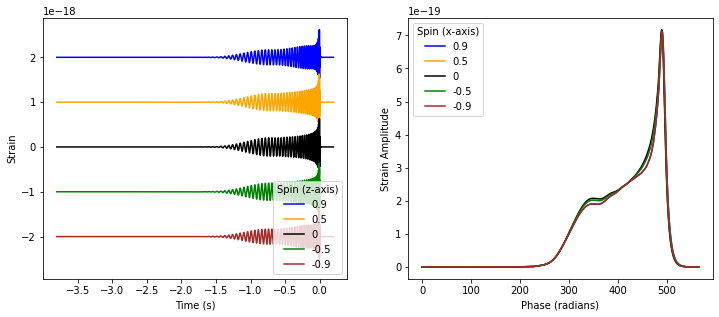
\includegraphics[width=\textwidth]{SNR29.png}}
    \caption{\label{fig:timechip} Time domain GW signal for a BBH of $m_1 = m_2 = 30 M_\odot$ with $0$ aligned spin and varying precession spin magnitudes.}
\end{figure}

Interestingly, as seen in Figure \ref{fig:timechip} there seems to be almost negligible change in the GW signal for varying precession spins, although positive precessing spins have marginally higher strain amplitudes. However, large variance in GW signal strength is still created, as seen in Figure \ref{fig:relsnr}. Whereas the effect of varying aligned spin is comparable for different mass ratios, the effect of varying precession spin is surprisingly different, especially at low $q$. \\

\begin{figure}[!htb]
    \center{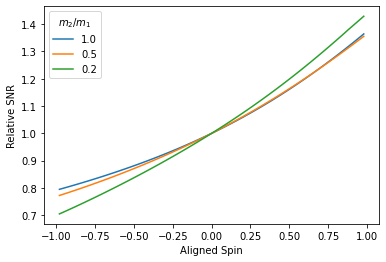
\includegraphics[width=2.5in]{SNR31.png} 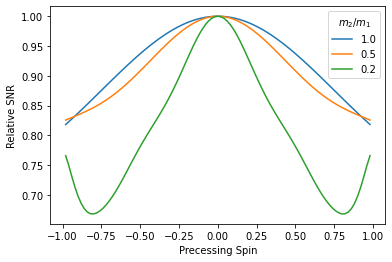
\includegraphics[width=2.5in]{SNR32.png}}
    \caption{\label{fig:relsnr} SNR of a BBH GW signal of $m_1 = 50 M_\odot$ and varying $m_2$ for different aligned spins and precessing spins, relative to the $0$ spin signal; $m_1$ and $m_2$ are assumed to have the same spin.}
\end{figure}

To ensure that the effective spin ($\chi_\text{eff}$) and effective precession spin ($\chi_\text{p}$) are a good approximant to the actual spin, we compare the SNR of various BBH inspirals with their original component masses and with the reduced parameter approximantions given by Eq. (4) and (5). We find that for the vast majority of spin combinations, accuracy is maintained to around a $\pm 10\%$ difference, with exceptions at unusually large spin magnitudes and low mass ratios, as illustrated in Figure \ref{fig:spincomps}. \\

\begin{figure}[!htb]
    \center{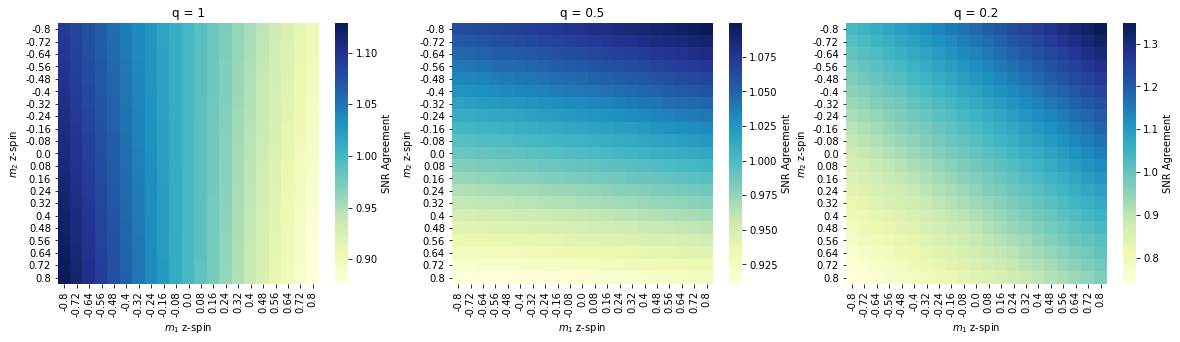
\includegraphics[width=\textwidth]{SNR33.png} 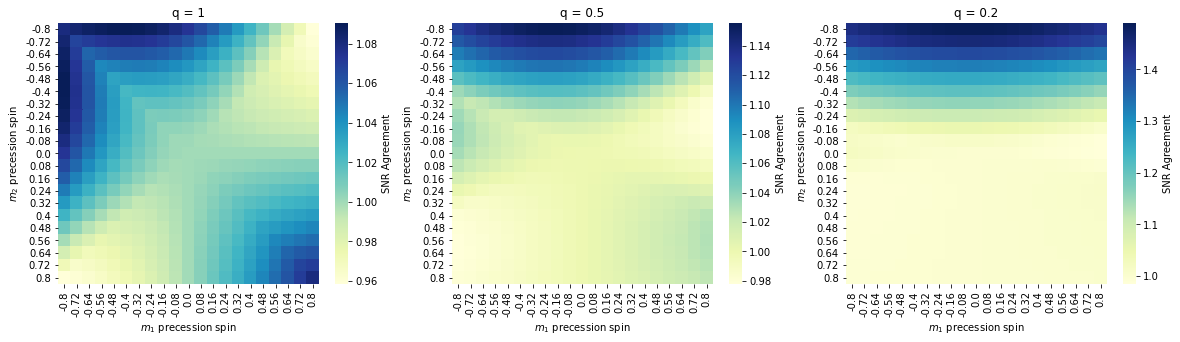
\includegraphics[width=\textwidth]{SNR34.png}}
    \caption{\label{fig:spincomps} Relative SNR of a BBH GW signal of $m_1 = 50 M_\odot$ and varying mass ratios using the reduced parameter approximation rather than component spins for (top) $\chi_\text{eff}$ and (bottom) $\chi_\text{p}$; values over 1 indicate an overestimation.}
\end{figure}

We now calculate the probability distribution of $\chi_\text{eff}$ and $\chi_\text{p}$ across the entire BBH population. Using Eq. (7) for the $\chi_\text{eff}$ distribution and an (arbitrarily chosen) Gaussian distribution with $\mu = 0.2$, $\sigma = 0.3$ for the $\chi_\text{p}$ distribution, we see in \ref{fig:spinhist} that most BBHs fall comfortably in the range at which the reduced parameterization accurately captures the GW signal strength. \\

\begin{figure}[!htb]
    \center{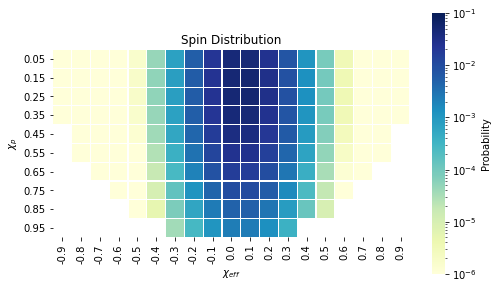
\includegraphics[width=3.5in]{SNR35.png}}
    \caption{\label{fig:spinhist} Probability distribution of BBH mergers over $\chi_\text{eff}$ and $\chi_\text{p}$, calculated in bins of 0.1 (axis ticks represent midpoints of bins). Gaussian distributions are independently normalized before taking out all bins with $\chi > 1$; the entire distribution is normalized again such that $\iint \chi d \chi_\text{eff} d \chi_\text{p} = 1$ }
\end{figure}

\begin{figure}[!htb]
    \center{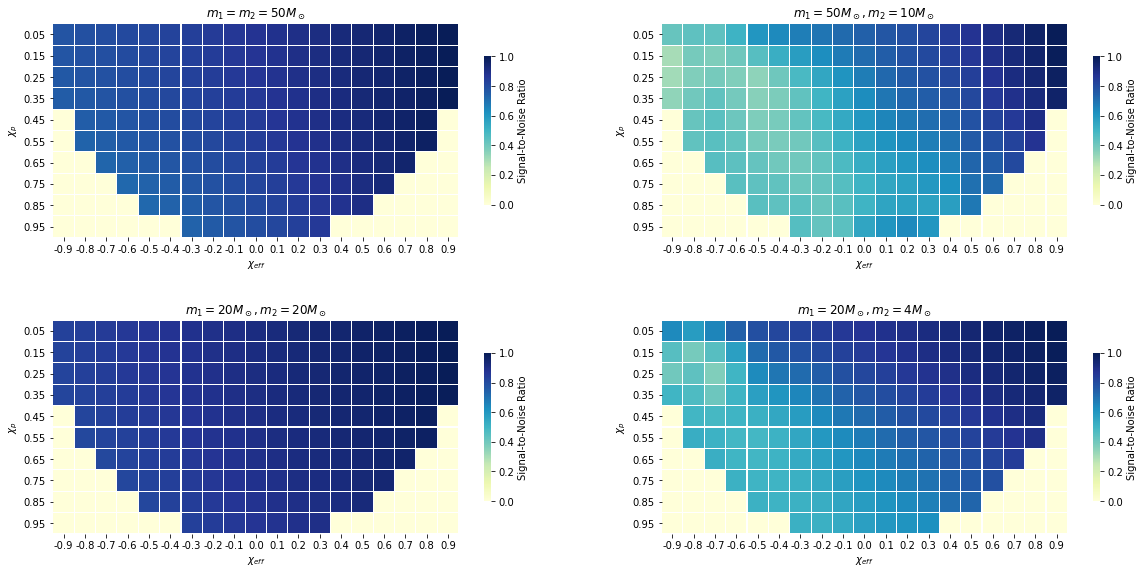
\includegraphics[width=\textwidth]{SNR36.png}}
    \caption{\label{fig:spinrel} SNR of various BBH GWs across the spin distribution as a fraction of the maximum SNR produced by one of the $(\chi_\text{eff}, \chi_\text{p})$ combinations}
\end{figure}

We investigate whether a simple analytical approximation can be calculated for the effect of varying effective aligned and precession spins on BBHs across the full spectrum of primary masses and/or mass ratios in Figure \ref{fig:spinrel}. Supposing that there are 20 primary mass bins, 20 mass ratio bins, 20 $\chi_\text{eff}$ bins, and 10 $\chi_text{p}$ bins, then the approximate time necessary to calculate the maximum distance of observation for all $(m_1, q, \chi_\text{eff}, \chi_\text{p})$ combinations is 
\begin{equation}
    (20 \times 20 \times 20 \times 10) \times (75 \text{ iterations}) \times (0.4 \text{ s/iteration}) \approx 28 \text{ days}
\end{equation}
Thus, it is clear that any analytical approximations would be extremely valuable. Unfortunately, as seen in Figure \ref{fig:spinrel} there appears to be significant variation in the effect of spin on GW signal strength even when holding either $m_1$ or $q$ constant. 

\end{document}